\documentclass{article}
\usepackage[utf8]{inputenc}
\usepackage{graphicx}
\usepackage{float}
\usepackage{epsfig}
\usepackage{blindtext}
\usepackage{graphicx}
\usepackage[T1]{fontenc}
\usepackage{amsmath}

\title{MATH 444 PS5}
\author{Connor Wolfe}
\date{April 2017}

\begin{document}

\maketitle

\section*{Introduction}
This problem set applies the text mining skills from class with previous algorithms in order to interpret genetic codes.  We will analyze a fragment of the genomic sequence of the bacterium \textit{Caulobacter Crescentus}.  To do so we use the matlab program 'LoadSeq.m' to read the Fasta-file 'ccrescentus.fa'.  We store the genetic sequence in the variable genseq as follows:
\begin{equation}
genseq=LoadSeq('ccrescentus.fa');
\end{equation}
We will break genseq into documents of length L which store words of length k.  We can see that since there are 4 letters, the number of words in the dictionary will be $4^k$. 
\\In the following sections we will first first visualize the term document matrices with varying values of L and k.  Then we will fix L=300 and k=3 to perform clustering, PCA, NMF, and other algorithmic techniques to analyze this term document matrix. 

\section*{1.c: Varying L and k}
We create various term document matrices by varying L and k and , and then center the data, compute the first two principal components, and then plot them.   We will thus see how the different values affect the visualization of data.

\subsection*{Vary k}
We will explore the PCA plots for k values from 1:6 and L=300.  To do so, we first compute a cell A which contains these 6 term document matrices.  I store this cell as 'TDM\_L\_300.mat' because it is time-consuming to compute.  Then, I iterate through the 6 term document matrices, compute their PCA.  To do so, first I center the matrix, and then compute the SVD.  Finally, I find the first two principal components as:
\begin{equation}
    Z=U(:,1:2)'*X;
\end{equation}

I then plot the first two principal components which we see for all 6 plots term document matrices in figure(1)

\begin{figure}[H]
    \centerline
    {
    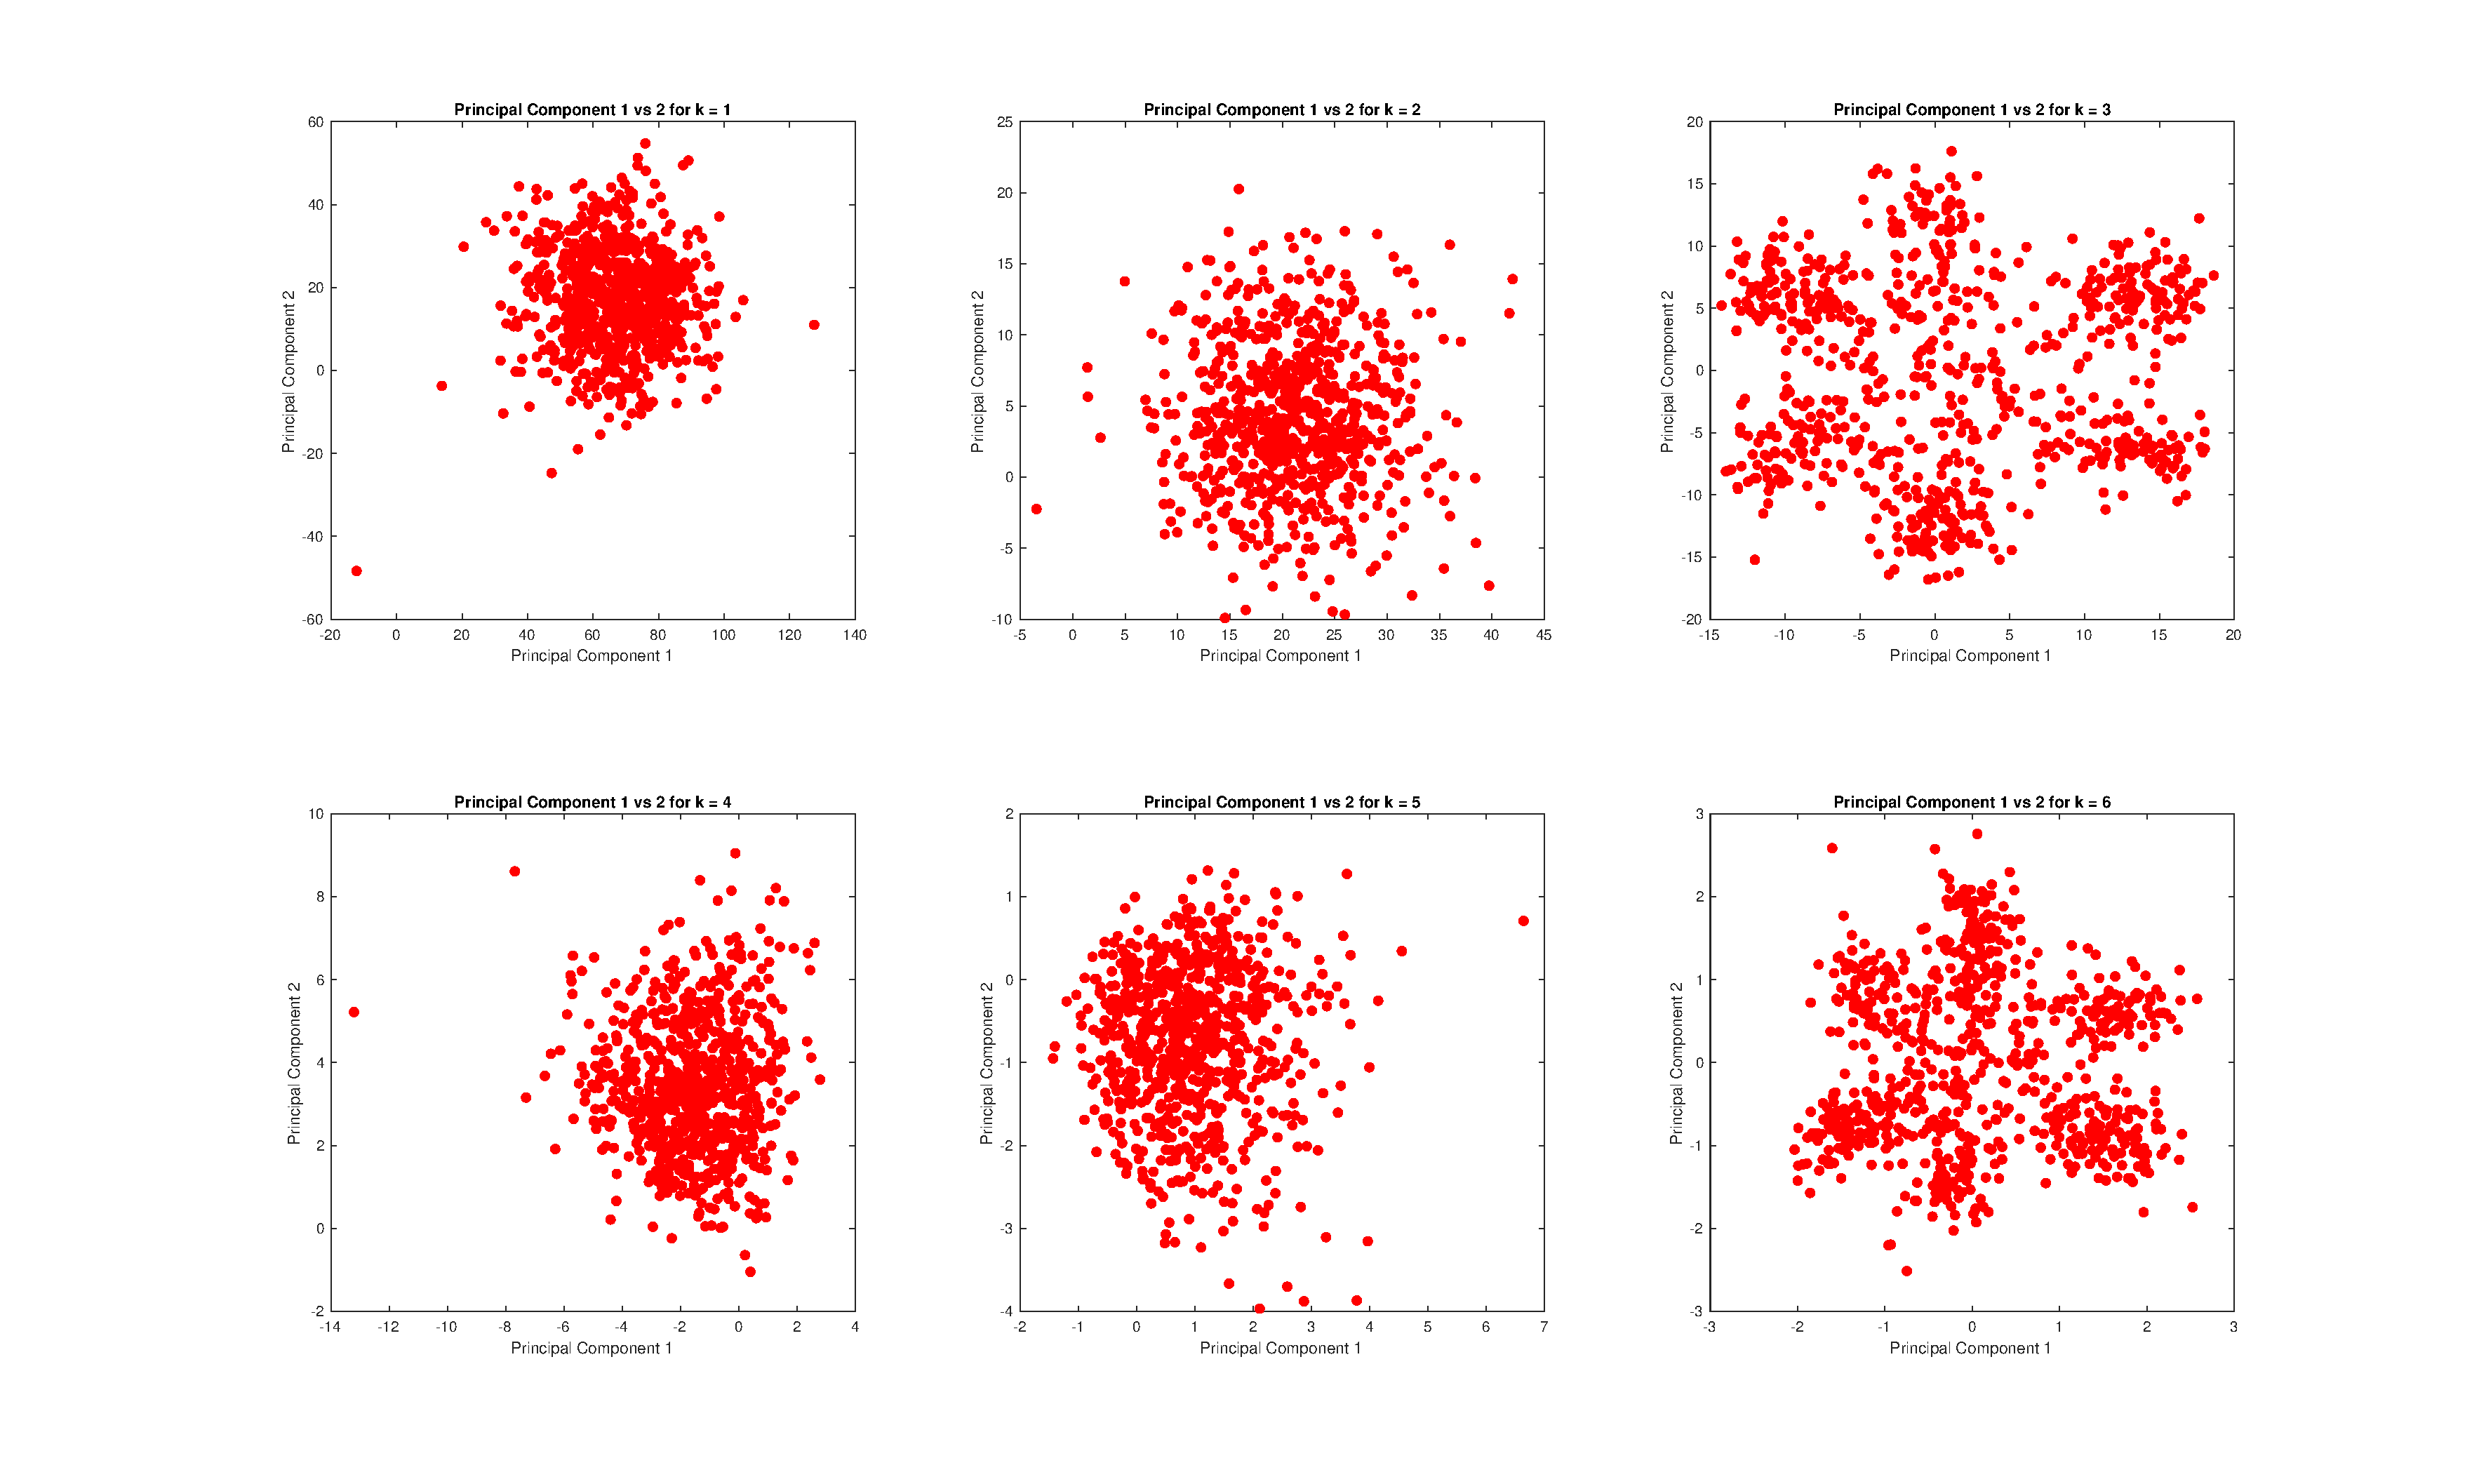
\includegraphics[width=17.5cm, height=8cm]{c_k_vary}
    }
    \caption{\label{fig:my figure} A plot of the first two principal components of the term document matrices for word length values k= 1:6.  We can clearly see the data clusters best at 3, the length of a codon. 6 seems to cluster well also, perhaps because it is a multiple of 3.}
\end{figure}

We can see that the data clusters rather well when k=3 or 6, but not for other k.  It makes sense that the clusters would be most visible when the word length equals the length of a codon, or a multiple of it.

\subsection*{Vary L}
We will now fix k=3 and explore how the PCA plots look for various lengths of documents in the term document matrix.  We will explore L= [100 200 400 500 1000] and lastly L=300 but with the first 5 characters of the string removed to test if the plot is sensitive to where we begin the document. 
\\We do the same analysis as before in computing the first two principal components and plotting them.  We see this data in figure (2).  

\begin{figure}[H]
    \centerline
    {
    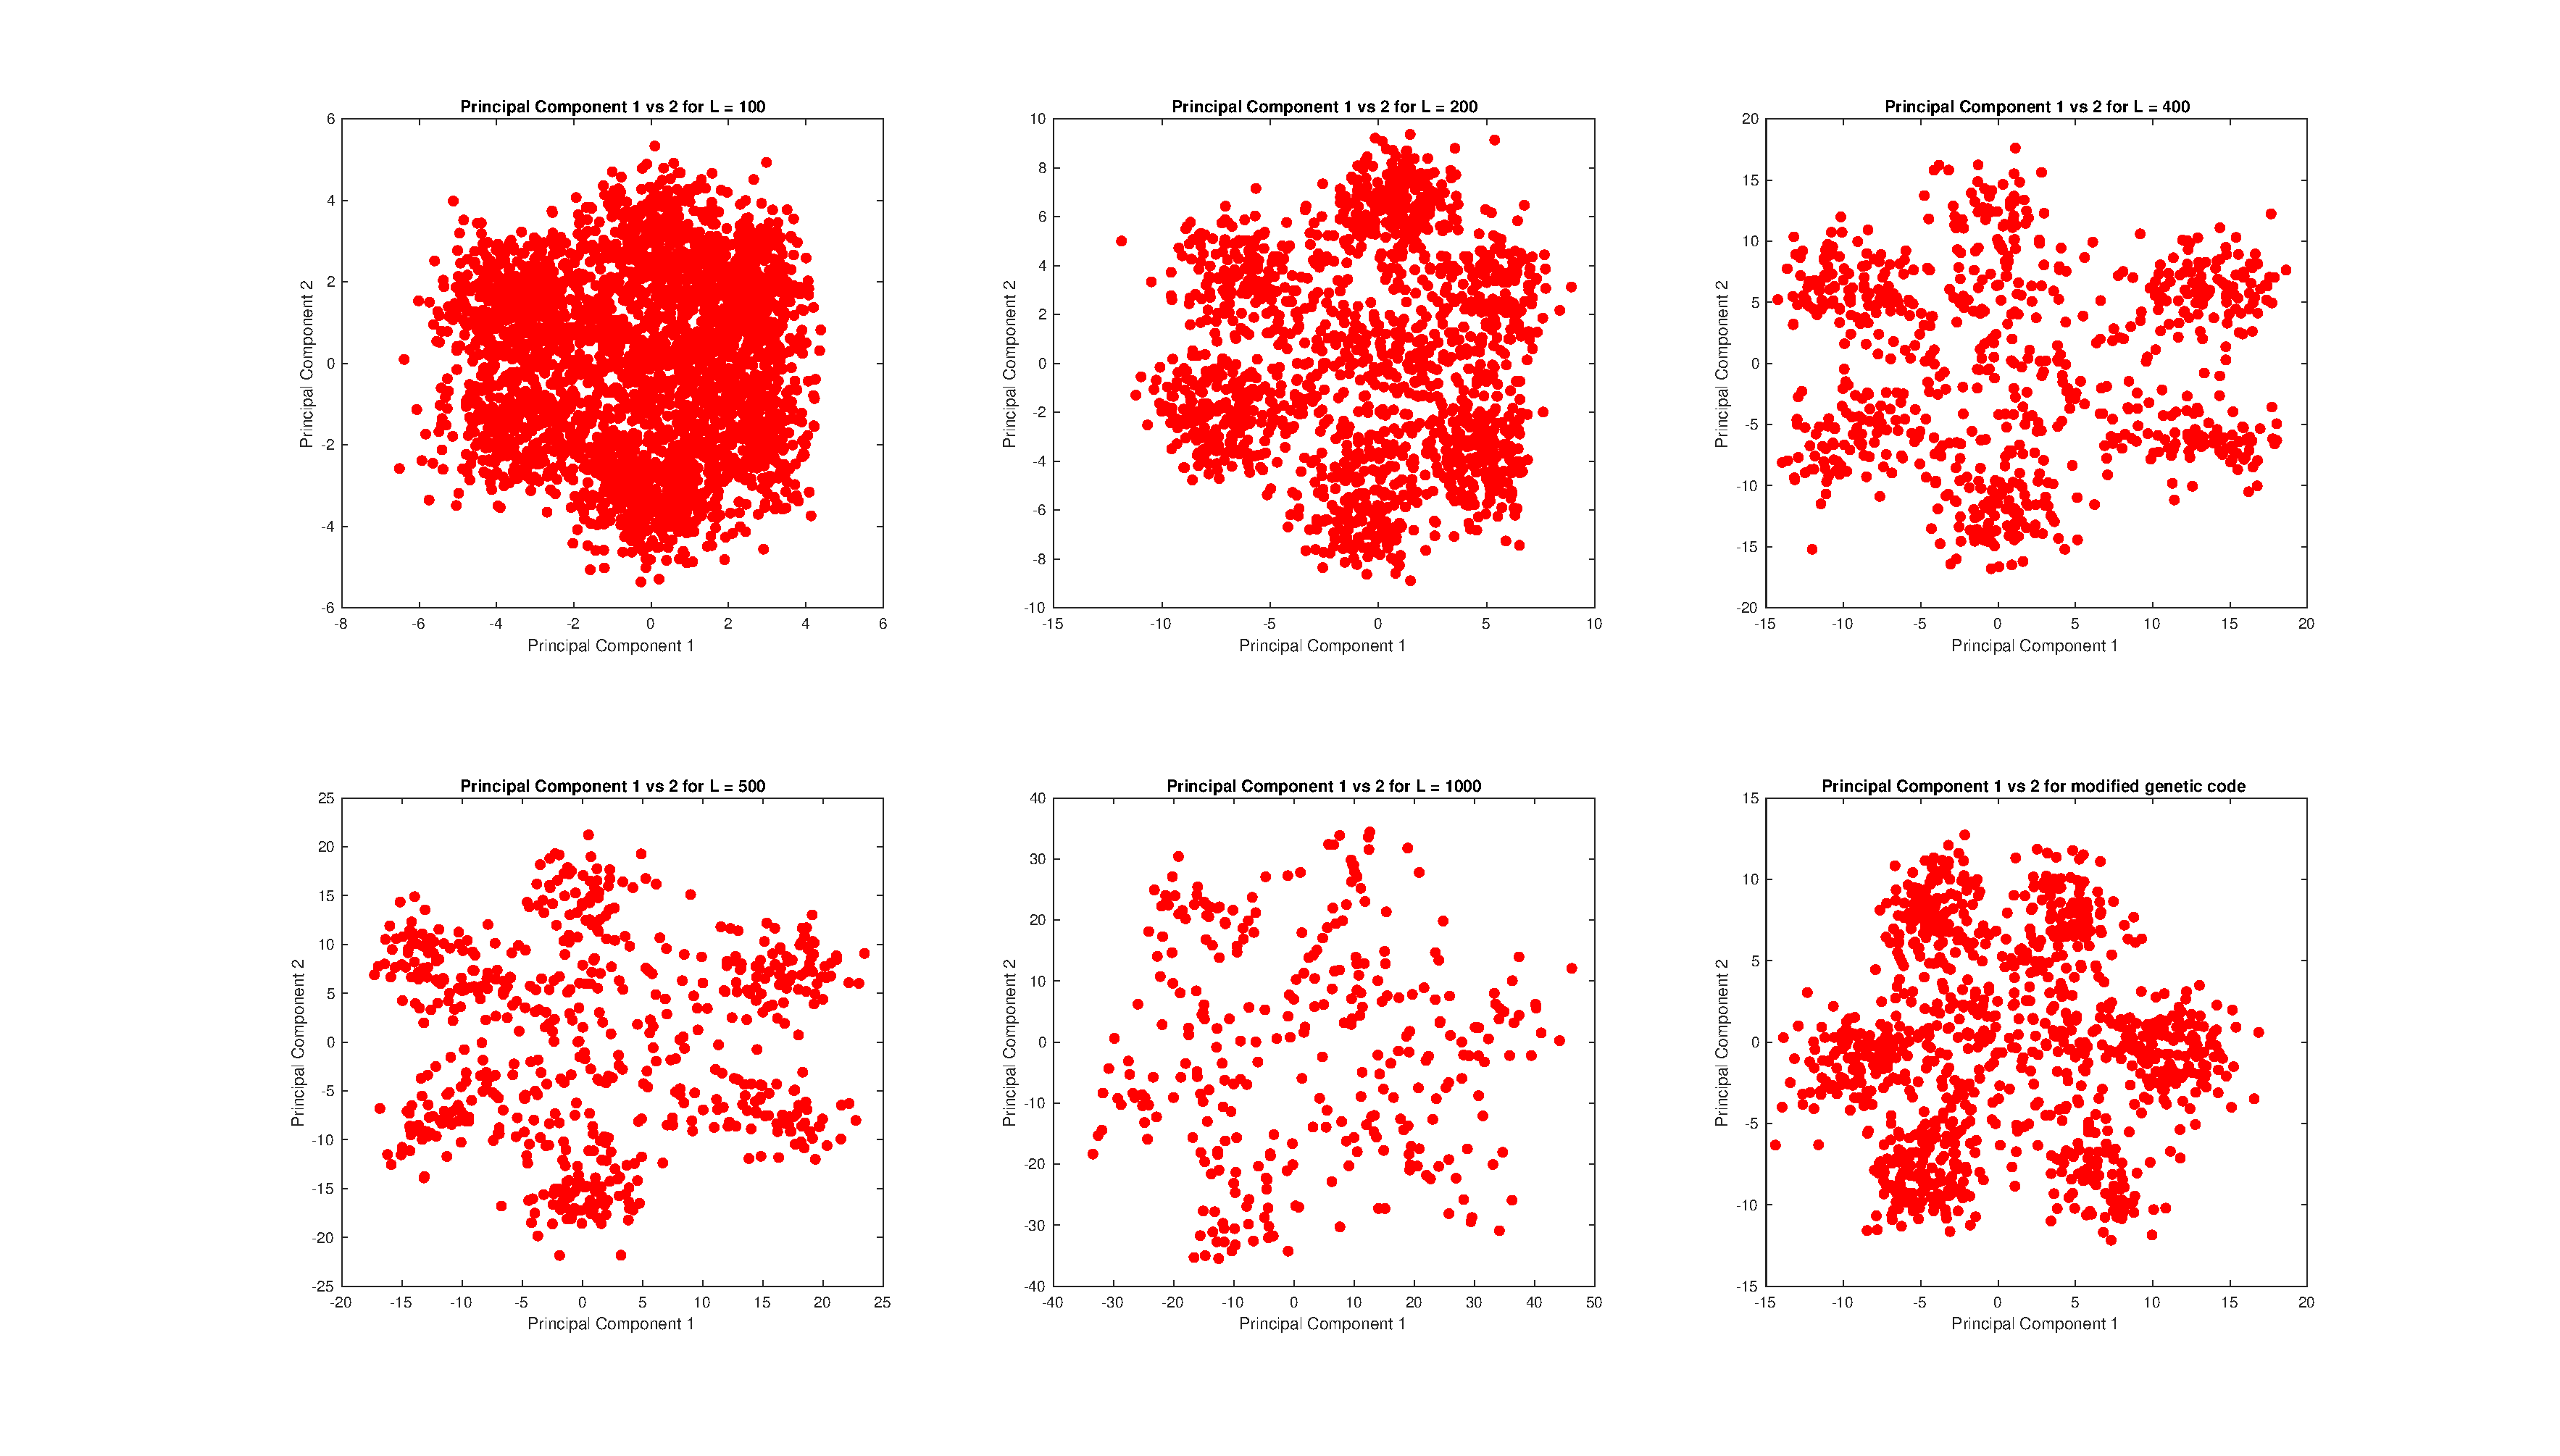
\includegraphics[width=17.5cm, height=8cm]{c_L_vary}
    }
    \caption{\label{fig:my figure} A plot of the first two principal components of the term document matrices for various document lengths/start points. We see the cluster shape preserved, but scaled poorly.  At values closer to L=300 it is most visible}
\end{figure}

The cluster shape is visible, but the scale is poor which makes it less clear.  As L increases from 100 to 1000, we see the points spread out into clusters, with most clear clusters as L approaches 300.  Changing the starting point as in plot 6 will actually show the clearest cluster as k=3 and L=300 here, only the starting character is changed.  

\section*{1.d: Clustering}

In this section we will run a clustering algorithm to classify each data point. Then we will plot the first two principal components again, but this time coloring the points by cluster.  We will fix k=3 and L=300 for this section as this shows the best clusters of data. The PCA plot shows that the optimal number of clusters is 6, which we will send to our clustering algorithm 
\\
First we will load the term document matrix corresponding to k=3 and L=300.  Then, we call k-medoids to return the indices the data for each of the 6 clusters.  We then calculate the PCA as before.  Lastly, we plot the first two principal components of each cluster in a different color, all superimposed on the same graph.  The results are shown in figure 3.

\begin{figure}[H]
    \centerline
    {
    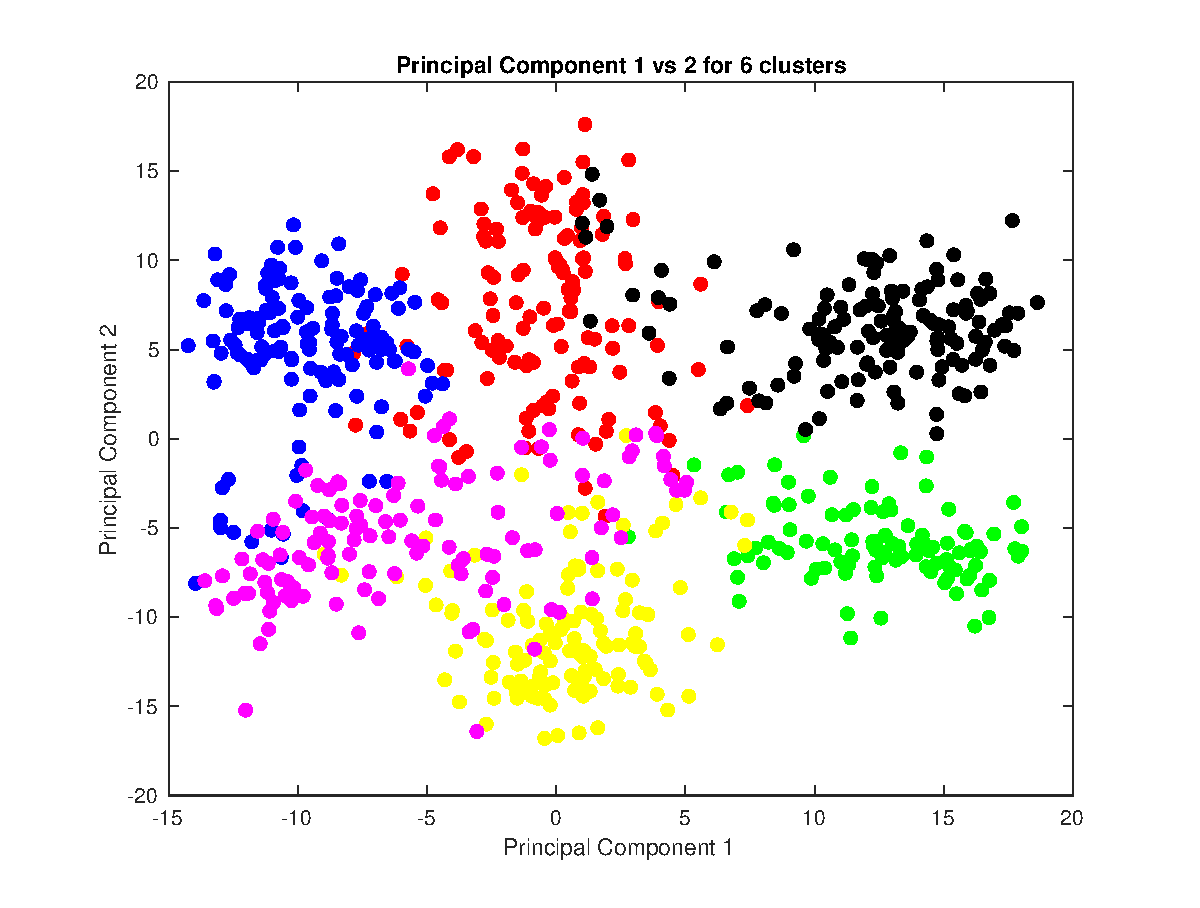
\includegraphics[width=17.5cm, height=8cm]{d_clusters}
    }
    \caption{\label{fig:my figure} A plot of the first two principal components of the term document matrix for L=300, k=3.  The colors correspond to the 6 clusters found when running k-medoids}
\end{figure}


\section*{1.e: NMF}
In this section we compute the NMF of the uncentered term document matrix. We will run ANLS with k=6 (the number of clusters).  We then calculate the first two principal components of the 6 feature vectors W, and plot these principal components over the principal components of the entire data set.  The goal is that each principal component of W would correspond to one cluster.  However, as we see in figure (4), the black dots which correspond to the principal components of W do not represent each cluster well.

\begin{figure}[H]
    \centerline
    {
    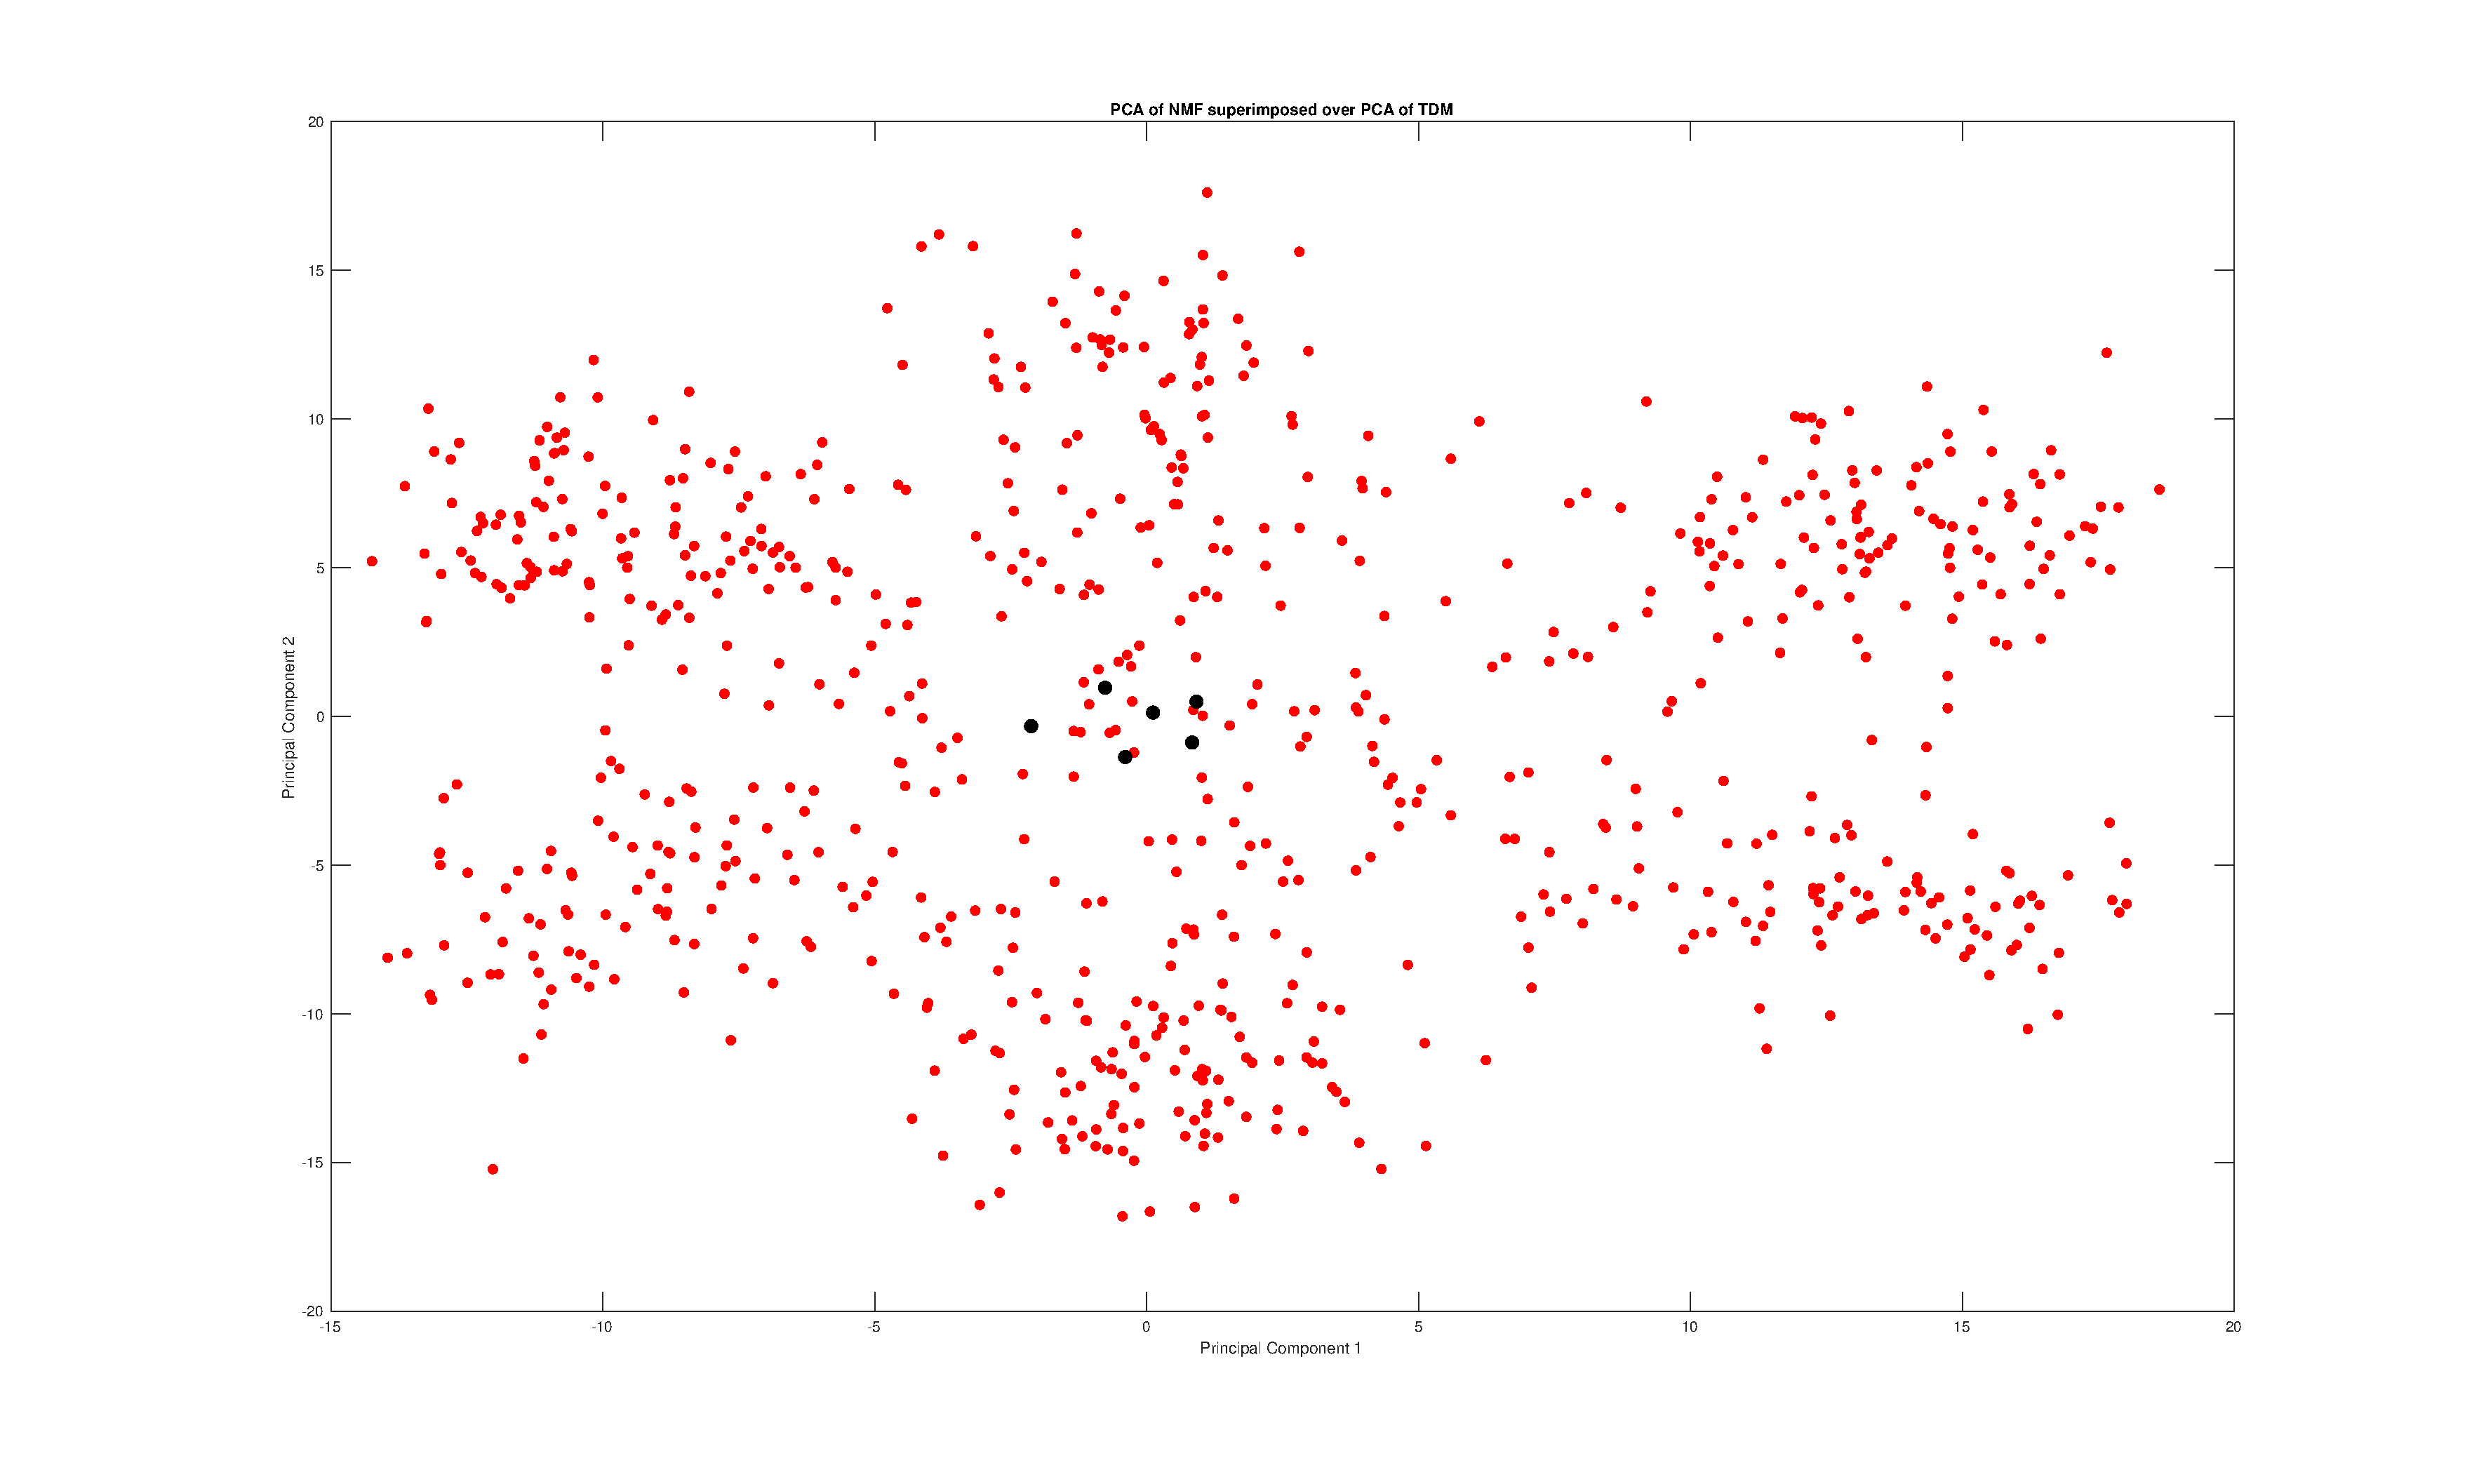
\includegraphics[width=17.5cm, height=8cm]{e_no_lines}
    }
    \caption{\label{fig:my figure} A plot of the first two principal components of the 6 feature vectors found in ANLS superimposed over the first two principal compoenents of the term document matrix for k=3, L=300.  Note that the principal components of W do not seem to represent the clusters well. }
\end{figure}

\\ It is possible, we realized that the principal components of W do represent the matrix well, the scaling just might be poor. In order to analyze this, we explore two methods.  First, we compute the voronoi plot of the 6 principal components to see if they capture the clusters well.  We see this analysis in figure (5).

\begin{figure}[H]
    \centerline
    {
    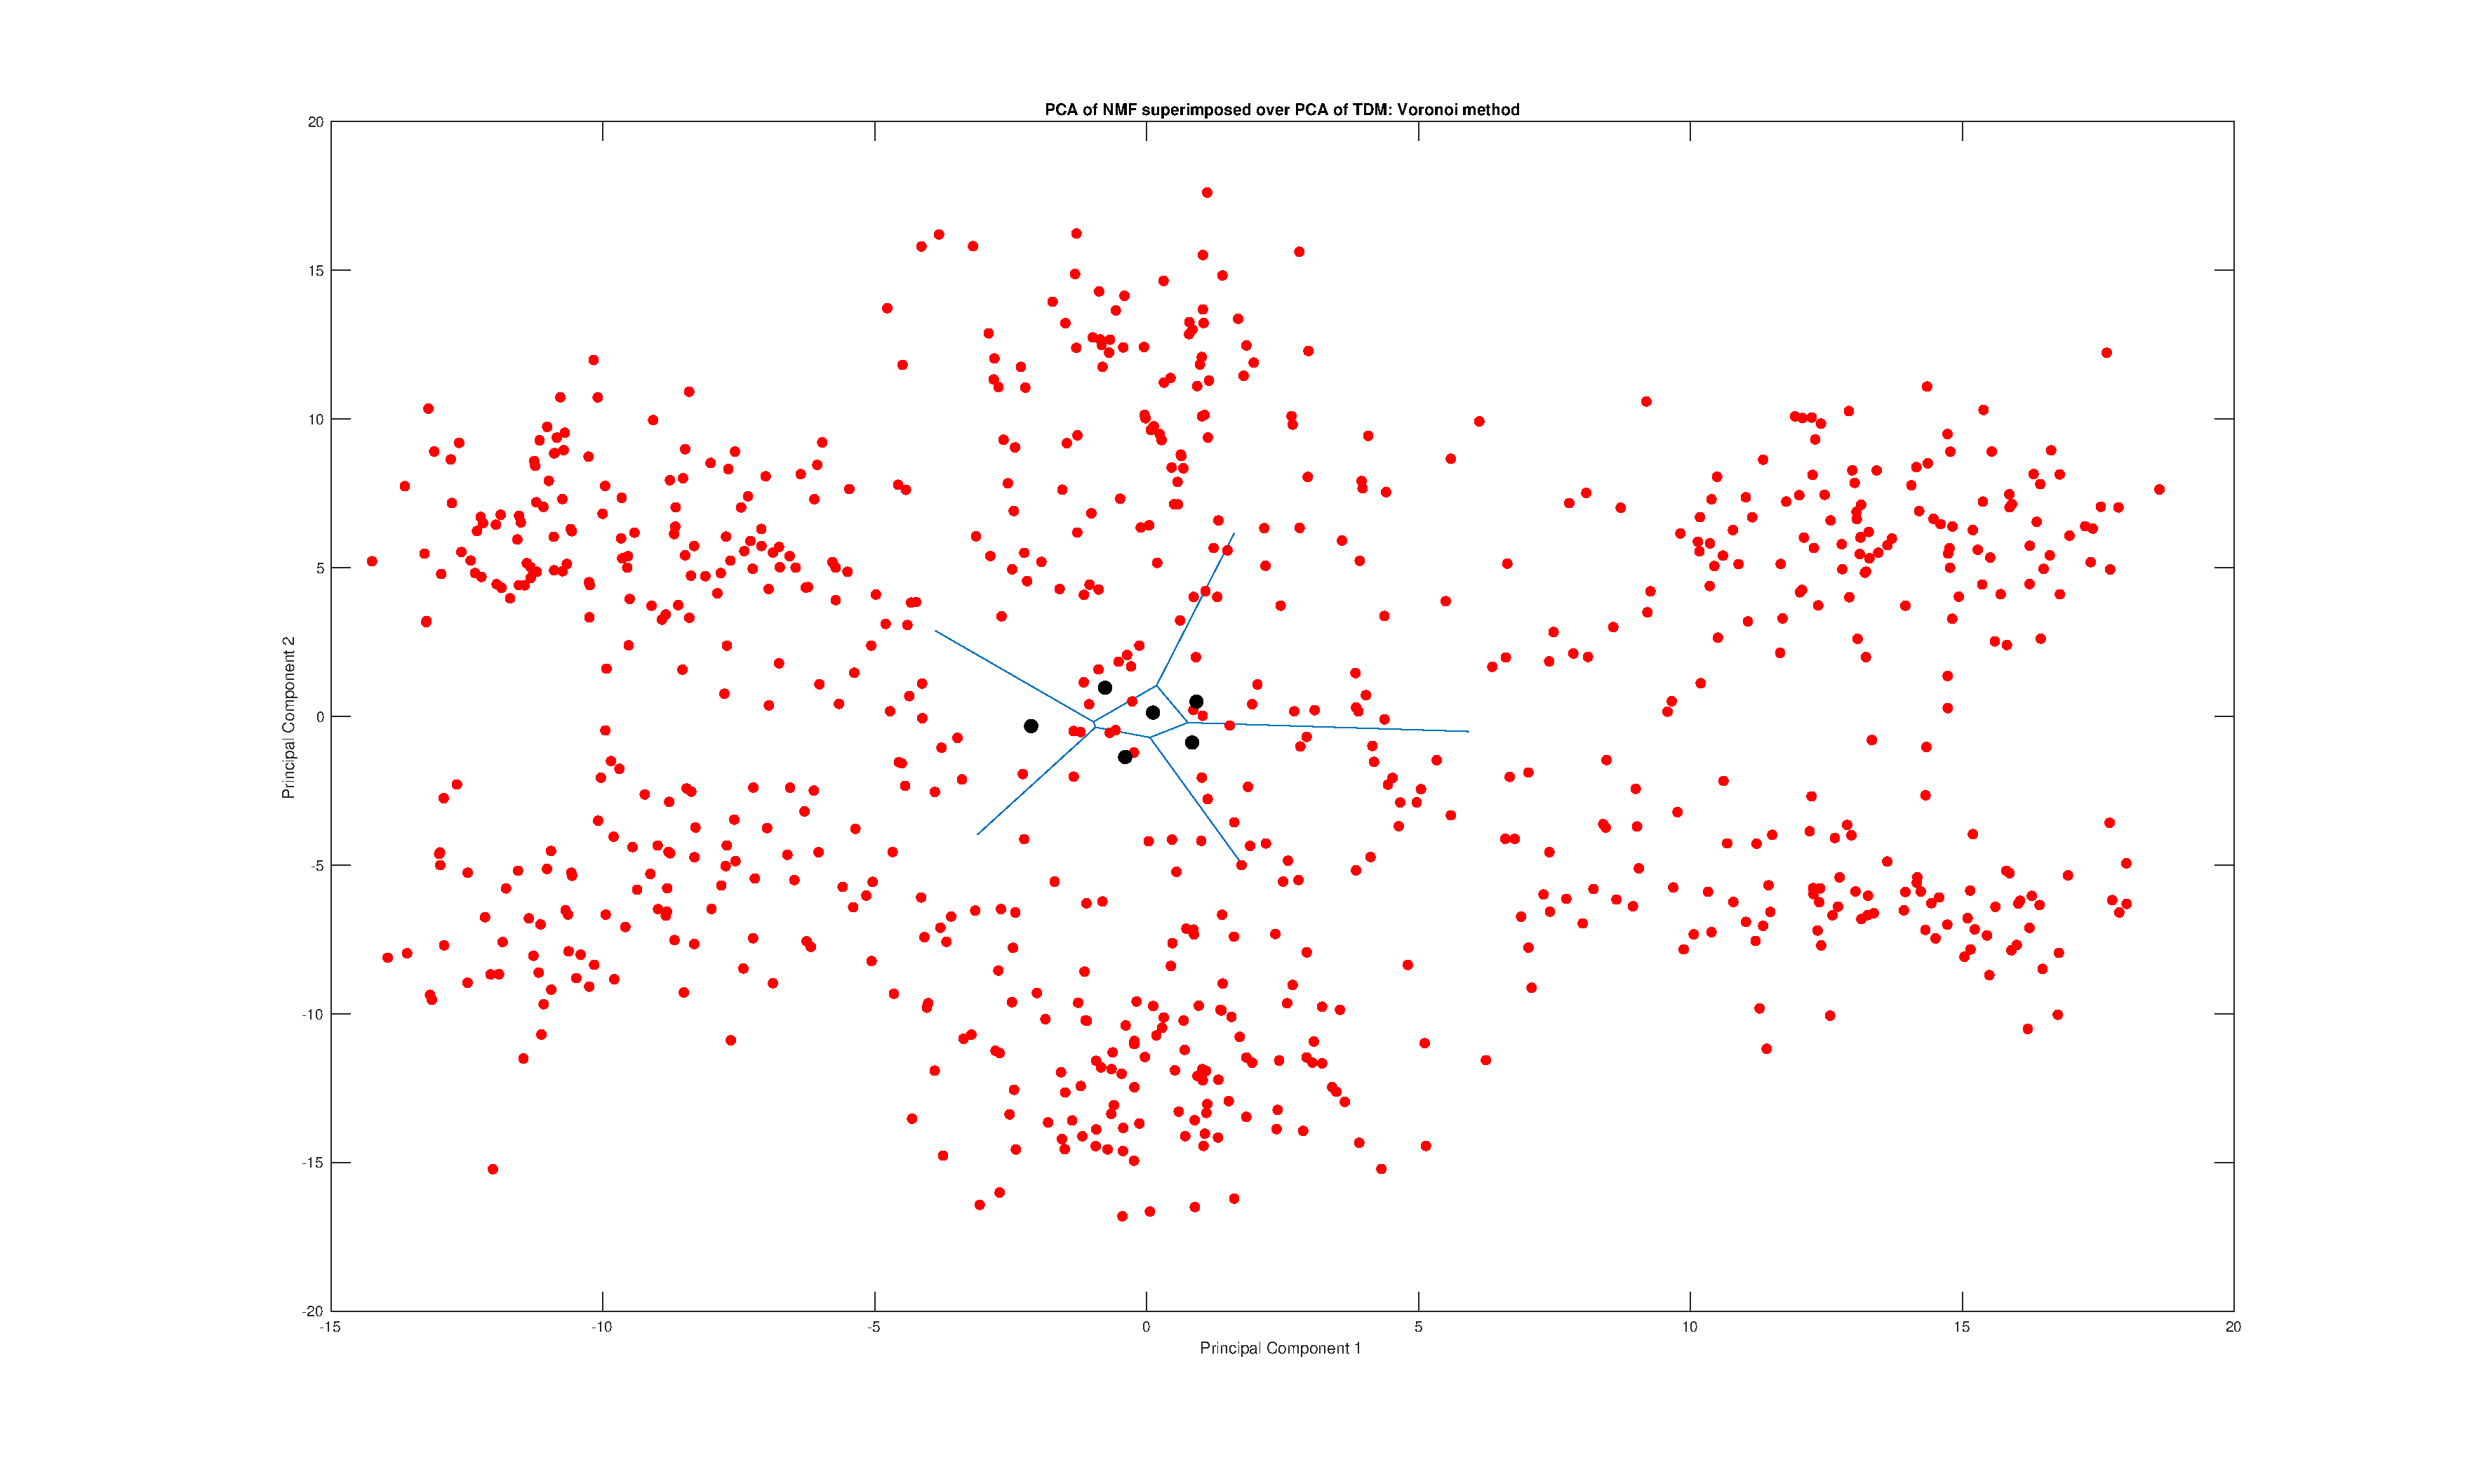
\includegraphics[width=17.5cm, height=8cm]{e_voronoi}
    }
    \caption{\label{fig:my figure} A plot of the voronoi diagram of the principal components of the 6 feature vectors from ANLS superimposed over the principal components of the term document matrix.  The plot actually captures the clusters rather well, better than it appeared, but only sees 5}
\end{figure}

We also try to consider the 6 points as vectors and extend them out from the origin in figure (6)

\begin{figure}[H]
    \centerline
    {
    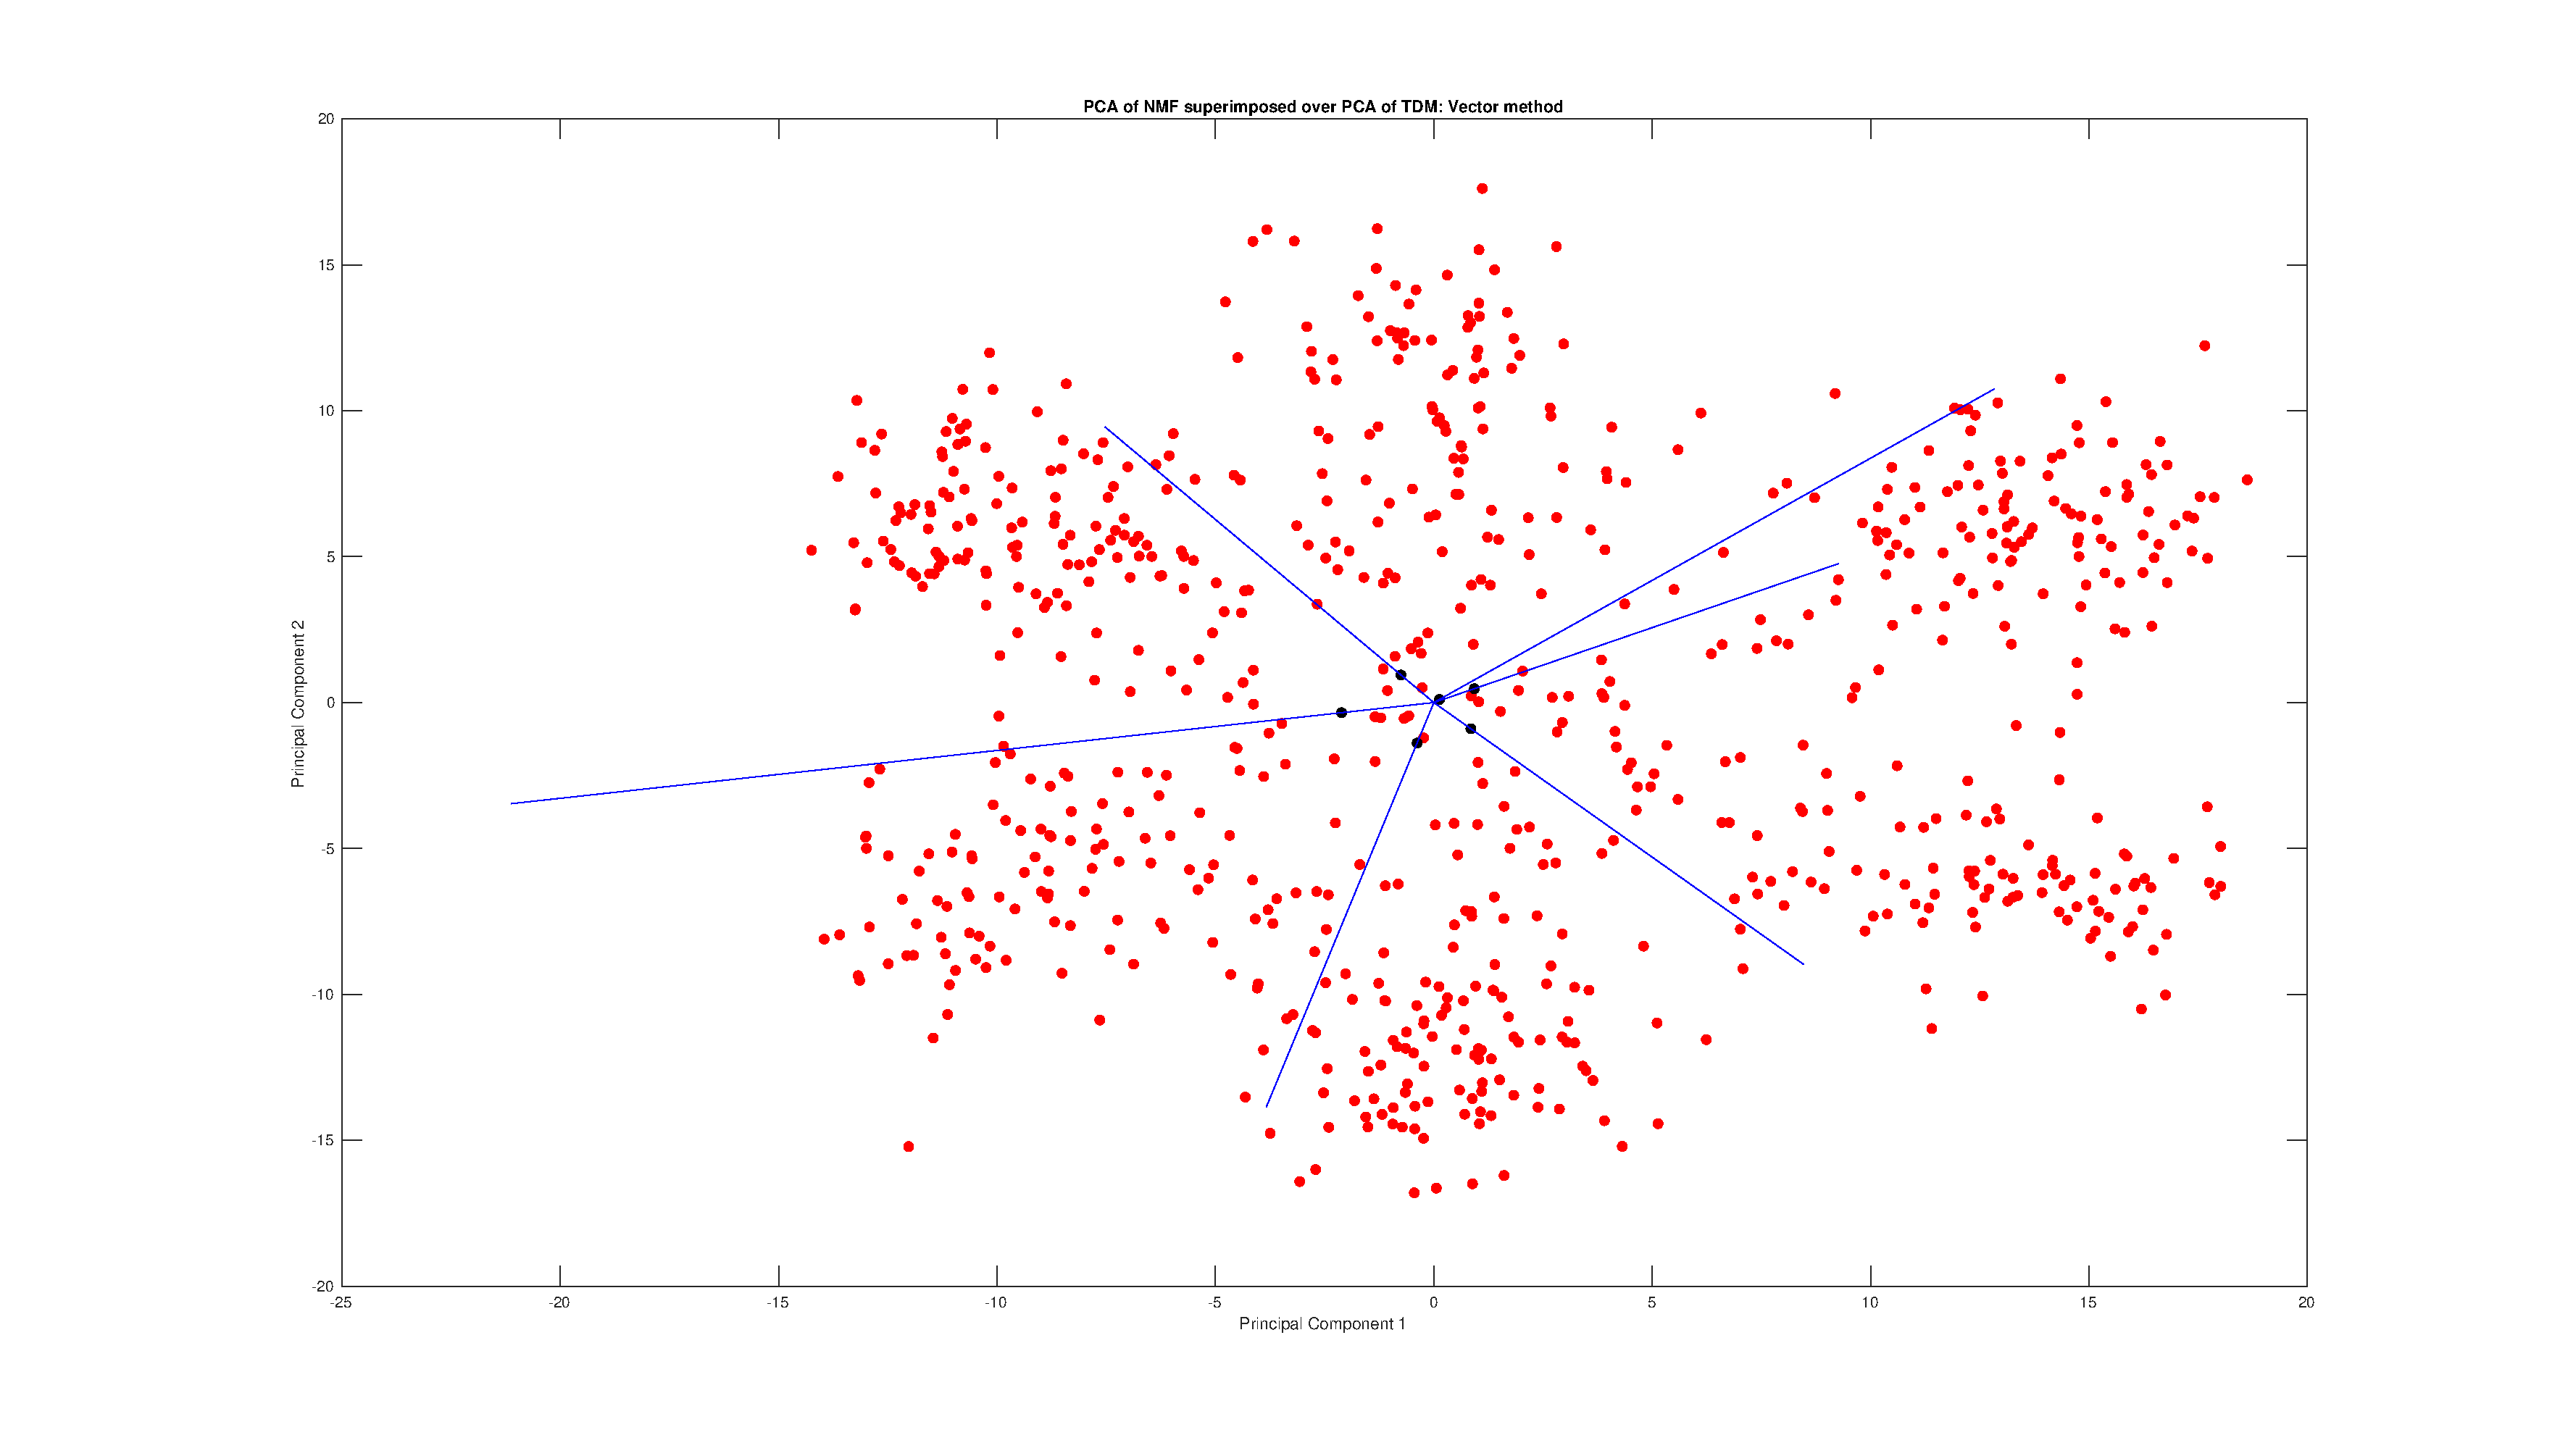
\includegraphics[width=17.5cm, height=8cm]{e_vector}
    }
    \caption{\label{fig:my figure} A plot of the vectors of the principal components of the 6 feature vectors from ANLS extended from the origin superimposed over the principal components of the term document matrix.  The plot actually captures the clusters rather well, but misses the distinction between the two rightmost clusters}
\end{figure}

The voronoi diagram and vector method show that the principal components of W captured the data far better than expected and are a decent representation of the clusters.

\section*{1.f: Identify Clusters}
This section asks us to compute the angle between the medoids of each cluster and each term document vector.  We then have 6 different angles between each vector and the medoids, and we find the index of the medoid which yields the maximum angle.  We classify the data vector to this medoid.  We then explore how well these classifications compare to the clustering classifications.

\\
First, we run k-medoids to obtain the 6 clusters.  then we create a matrix cos (763 x 6) to store the angle between each data vector and each medoid.  We then iterate through the 6 medoids and every data vector, and compute the cosine of the angle following equation (3) which computes the cosine between vectors q and a as their vector product divided by the product of their euclidean norms.
\begin{equation}
        cosin(q, a)= \frac{q'*a}{||q||*||a||}
\end{equation}

In matlab, this translates equation (4) where j=1:763 for the data vectors and i=1:6 for the clusters.  We multiply the data vector transpose by the medoid and divide by the product of their euclidean norms.

\begin{equation}
        cos(j,i)=  \frac{X(:,j)'*X(:,m_{ind}(i))}{(norm(X(:,j), 2)*norm(X(:,m_{ind}(i)),2)} ;
\end{equation}

We then visualize the cosine between the data vectors and every plot using the clusters.  We want the cosine of the data vectors corresponding to the cluster we computed with to be highest, because the vectors in a given cluster should be more similar to the medoid than the other points. We see a plot of the cosines relative to all 6 clusters in figure (7).

\begin{figure}[H]
    \centerline
    {
    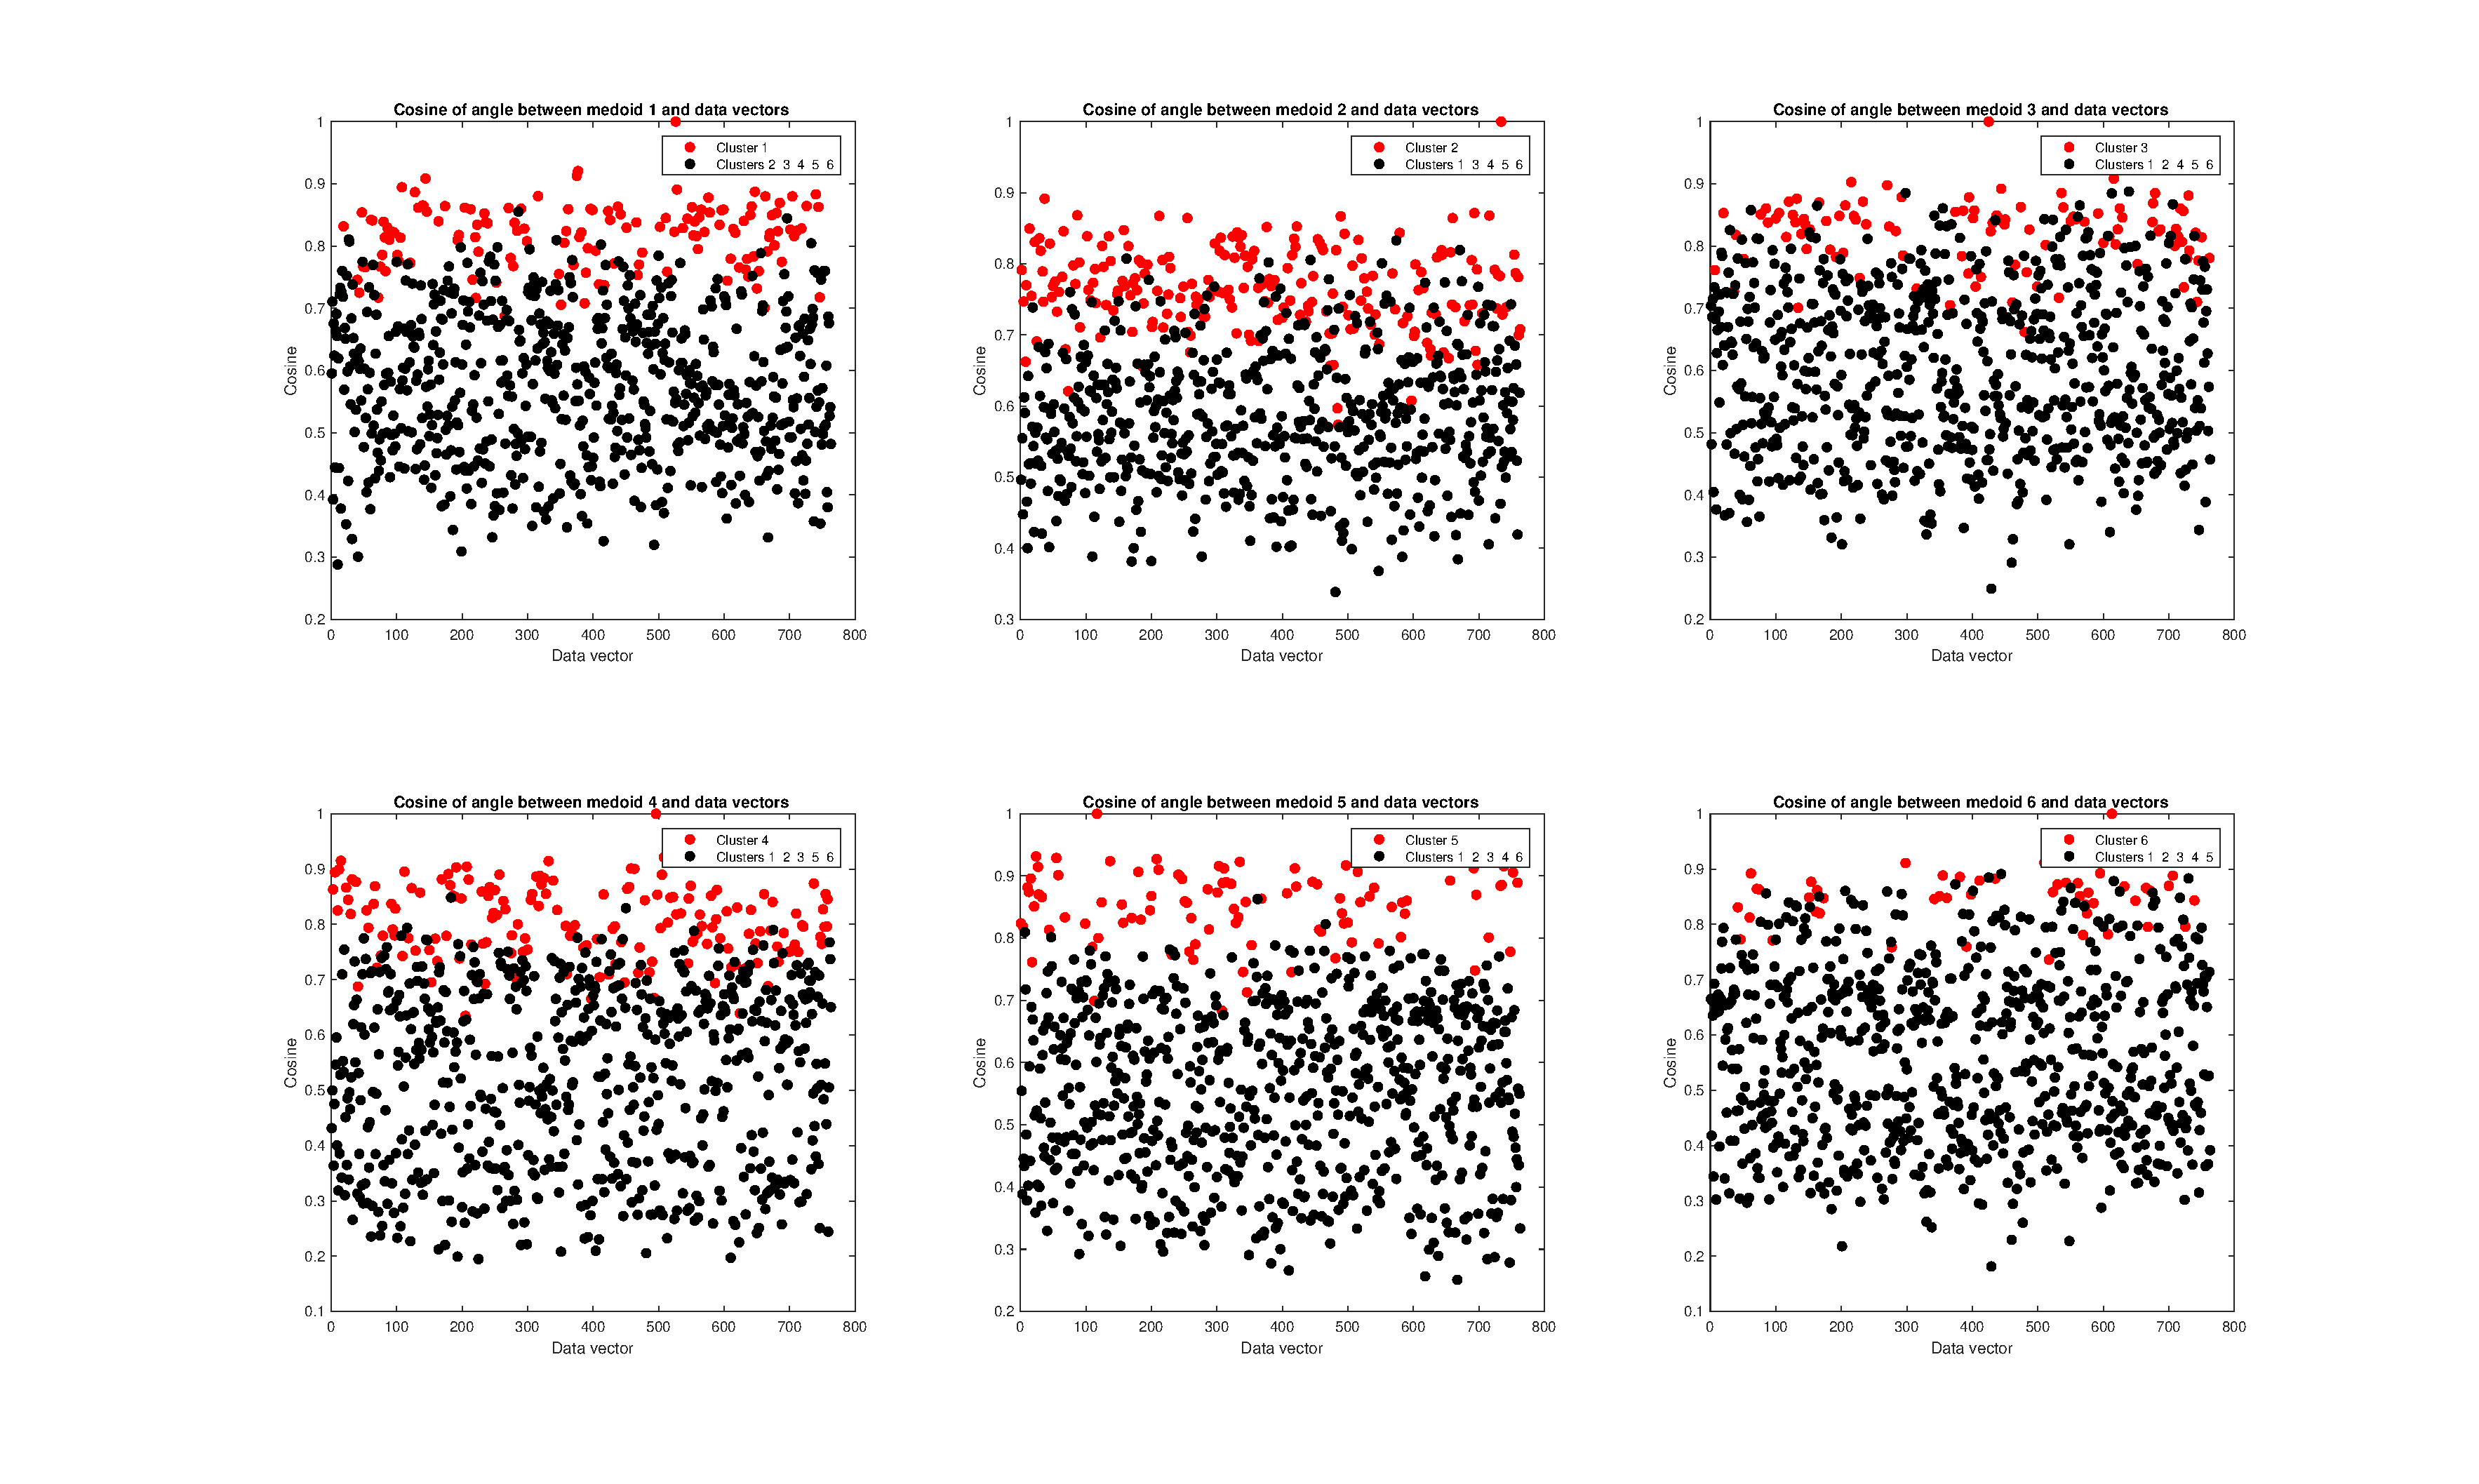
\includegraphics[width=17.5cm, height=8cm]{f_cosine}
    }
    \caption{\label{fig:my figure} A plot of the cosine between the data vectors and the six medoids.  The points in the cluster of the given medoid of each plot are in red, and the remaining points in black.  We see the points in the medoid's cluster have the highest cosine which makes sense because they should be most similar to the medoid}
\end{figure}

As we hoped, the points in red corresponding to the cosine between data vectors in the medoids cluster are highest.  This means that the points in a cluster are more similar to the cluster medoid than other points. Therefore if we used a medoid as a query we would clearly find the cluster well by finding the largest cosine between the query and the data points.

\end{document}
